\chapter{Introduction to Security Testing}
	\clearpage
	\section{The OWASP Testing Guide}
		{\bf OWASP:} The Open Web Application Security Project

		The OWASP Testing Project has been in development for many years. With this project, 
		we wanted to help people understand the what, why, when, where, and how of testing their 
		web applications, and not just provide a simple checklist or prescription of issues 
		that should be addressed. The outcome of this project is a complete Testing Framework, 
		from which others can build their own testing programs or qualify other people’s 
		processes. The Testing Guide describes in details both the general Testing Framework and 
		the techniques required to implement the framework in practice.

		\section{What, Why, When?}

		{\bf What is Testing?} \\
		What do we mean by testing? During the development life cycle of a web application, 
		many things need to be tested. The Merriam-Webster Dictionary describes testing as:
			\begin{itemize}
				\item To put to test or proof.
				\item To undergo a test.
				\item To be assigned a standing or evaluation based on tests.
			\end{itemize}
		Many outsiders regard security testing as a black art. This document’s aim is to
		change that perception and to make it easier for people without in-depth security 
		knowledge to make a difference.

		{\bf Why Testing?} \\
		This document is designed to help organizations understand what comprises a testing 
		program, and to help them identify the steps that they need to undertake to build 
		and operate that testing program on their web applications. 
		It is intended to give a broad view of the elements required to make a comprehensive 
		web application security program. 
		This guide can be used as a reference and as a methodology to help determine the gap 
		between your existing practices and industry best practices. 
		This guide allows organizations to compare themselves against industry peers, understand 
		the magnitude of resources required to test and maintain their software, or prepare for 
		an audit. 
		The technical details about how to test an application, as part of a penetration test or code review, will be covered in later chapters. 

		\clearpage
		{\bf When to Test?} \\ 
		Most people today don’t test the software until it has already been created and is in 
		the deployment phase of its life cycle (i.e., code has been created and instantiated 
		into a working web application). 
		This is generally a very ineffective and cost-prohibitive practice. One of the best 
		methods to prevent security bugs from appearing in production applications is to 
		improve the Software Development Life Cycle (SDLC) by including security in each of 
		its phases. 

		An SDLC is a structure imposed on the development of software artifacts. If an SDLC 
		is not currently being used in your environment, it is time to pick one! 
		The following figure shows a generic SDLC model: 

		\begin{figure} [H]
			\centering
			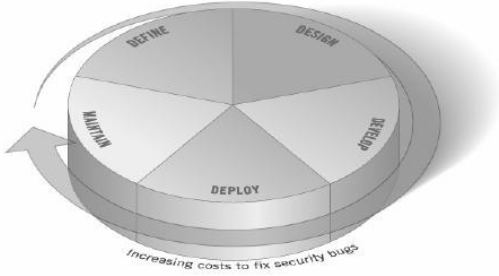
\includegraphics[scale=0.5]{pics/SDCL.png}
		\end{figure}


		{\bf What to Test?} \\
		It can be helpful to think of software development as a combination of people, process, 
		and technology. If these are the factors that "create" software, then it is logical 
		that these are the factors that must be tested. Today most people generally
		test the technology or the software itself. An effective testing program should 
		have components that test \\
		{\bf People} – to ensure that there is adequate education and
		awareness; \\ 
		{\bf Process} – to ensure that there are adequate policies and standards and 
		that people know how to follow these policies; \\ 
		{\bf Technology} – to ensure that the process has been effective in its implementation. 

		\clearpage
		\section{Principles of Testing}

			{\bf There is no silver bullet: } While it is tempting to think that a security 
			scanner or application firewall will either provide a multitude of defenses or
			identify a multitude of problems, in reality there are no silver bullets to the 
			problem of insecure software.

			{\bf Think strategically, not tactically: } The patch-and-penetrate model involves
			fixing a reported bug, but without proper investigation of the root cause. 
			This model is usually associated with the window of vulnerability:

				\begin{figure}[H]
					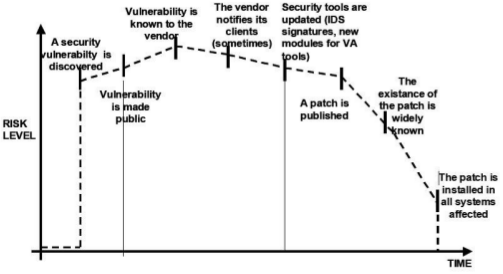
\includegraphics[scale=0.7]{pics/windowOfExposure.png}
				\end{figure}


			To prevent reoccurring security problems within an application, it is essential 
			to build security into the Software Development Life Cycle (SDLC) by developing
			standards, policies, and guidelines that fit and work within the development
			methodology. Threat modeling and other techniques should be used to help assign
			appropriate resources to those parts of a system that are most at risk.


			{\bf Test early and test often: } When a bug is detected early within the SDLC, 
			it can be addressed more quickly and at a lower cost. A security bug is no
			different from a functional or performance-based bug in this regard.


			{\bf Understand the scope of security:} It is important to know how much security 
			a given project will require. The information and assets that are to be protected
			should be given a classification that states how they are to be handled (e.g., Confidential, Secret, Top Secret). Security testing cost money! You have to
			prioritize what's important for your system. 

			\clearpage
			{\bf Develop the right mindset: } Successfully testing an application for security
			vulnerabilities requires thinking "outside of the box." Normal use cases will
			test the normal behavior of the application when a user is using it in the manner 
			that you expect. Good security testing requires going beyond what is expected and
			thinking like an attacker who is trying to break the application. This is one of 
			the reasons why automated tools are actually bad at automatically testing for
			vulnerabilities.

			{\bf Understand the subject: } One of the first major initiatives in any good 
			security program should be to require accurate documentation of the application. 
			The architecture, data-flow diagrams, use cases, and more should be written in 
			formal documents and made available for review. 

			{\bf Use the right tools: } While we have already stated that there is no silver 
			bullet tool. There is a range of open source and commercial tools that can 
			automate many routine security tasks. These tools can simplify and speed up the 
			security process. It is important to understand exactly what these tools can 
			and cannot do.

			{\bf The devil is in the details: } It is critical not to perform a superficial
			security review of an application and consider it complete. Care should be taken 
			to verify that every possible section of application logic has been tested, and 
			that every use case scenario was explored for possible vulnerabilities.

			{\bf Use source code when available: } While black box penetration test results 
			can be impressive and useful to demonstrate how vulnerabilities are exposed in
			production, they are not the most effective way to secure an application. 
			If the source code for the application is available, it should be given to the 
			security staff to assist them while performing their review. 
			It is possible to discover vulnerabilities within the application source that 
			would be missed during a black box engagement.

			{\bf Develop metrices: } An important part of a good security program is the 
			ability to determine if things are getting better. It is important to track
			the results of testing engagements, and develop metrics that will reveal the
			application security trends within the organization. 

			{\bf Document the test results: } To conclude the testing process, it is 
			important to produce a formal record of what testing actions were taken, 
			by whom, when they ware performed, and details of the test findings.


	\clearpage
	\section{Testing Techniques}

		This section presents a high-level overview of various testing techniques that 
		can be employed when building a testing program.

		\subsection{Manual Inspection and Reviews}
			Manual inspections are human-driven reviews that typically test the security
			implications of the people, policies, and processes, but can include inspection 
			of technology decisions such as architectural designs.
			By asking someone how something works and why it was implemented in a specific way, 
			it allows the tester to quickly determine if any security concerns are likely to 
			be evident. Manual inspections and reviews are one of the few ways to test
			the software development life-cycle process itself and to ensure that there is 
			an adequate policy or skill set in place. 
			As with many things in life, when conducting manual inspections and reviews we suggest you adopt a trust-but-verify model. 

			{\bf Advantages:}
			\begin{itemize}
				\item Requires no supporting technology
				\item Can be applied to a variety of situations
				\item Flexible
				\item Promotes teamwork
				\item Can be performed early in the SDLC
			\end{itemize}

			{\bf Disadvantages:}
			\begin{itemize}
				\item Can be time consuming
				\item Supporting material not always available
				\item Requires significant human thought and skill to be effective!
			\end{itemize}

		\clearpage
		\subsection{Threat Modeling}
			Threat modeling has become a popular technique to help system designers think 
			about the security threats that their systems/applications might face. 
			Therefore, threat modeling can be seen as risk assessment for applications. 
			In fact, it enables the designer to develop mitigation strategies for potential
			vulnerabilities and helps them focus their inevitably limited resources and 
			attention on the parts of the system that most require it.
			To develop a threat model, we recommend taking a simple approach.
			This approach involves:

			\begin{itemize}
				\item {\bf Defining and classifying the assets} – classify the assets into tangible and intangible assets and rank them according to business importance.
				\item {\bf Exploring potential vulnerabilities} - whether technical, operational, 
				or management.
				\item {\bf Decomposing the application} – how the application works, its assets,
				functionality, and connectivity.
				\item {\bf Exploring potential threats} – use threat scenarios and/or attack trees.
				\item {\bf Creating mitigation strategies} – develop mitigating controls for each of the threats deemed to be realistic.
			\end{itemize}

			{\bf Advantages:}
				\begin{itemize}
					\item Practical attacker's view of the system
					\item Flexible
					\item Early in the SDLC
				\end{itemize}

			{\bf Disadvantages:}
				\begin{itemize}
					\item Relatively new technique
					\item Good threat models don’t automatically mean good software
				\end{itemize}

		\clearpage
		\subsection{Source Code Review}
			Source code review is the process of manually checking a web application's source 
			code for security issues. Many serious security vulnerabilities cannot be detected 
			with any other form of analysis or testing. As the popular saying goes “if you
			want to know what’s really going on, go straight to the source." Almost all 
			security experts agree that there is no substitute for actually looking at the 
			code. All the information for identifying security problems is there in the code
			somewhere.

			{\bf Advantages:}
			\begin{itemize}
				\item Completeness and effectiveness
				\item Accuracy
				\item Fast (for competent reviewers)
			\end{itemize}
			{\bf Disadvantages:}
			\begin{itemize}
				\item Requires highly skilled security developers
				\item Can miss issues in compiled libraries
				\item Cannot detect run-time errors easily
				\item The source code actually deployed might differ from the one being analyzed
			\end{itemize}

		\clearpage	
		\subsection{Penetration Testing}

		Penetration testing has been a common technique used to test network security for 
		many years. It is also commonly known as black box testing or ethical hacking. 
		Penetration testing is essentially the “art” of testing a running application remotely,
		without knowing the inner workings of the application itself, to find security
		vulnerabilities. Typically, the penetration test team would have access to an 
		application as if they were users. The tester acts like an attacker and attempts 
		to find and exploit vulnerabilities. 
		Penetration testing tools have been developed that automate the
		process, but, again, with the nature of web applications their effectiveness is 
		usually poor. 

		Gary McGraw summed up penetration testing well when he said: \\
		{\bf “If you fail asummed penetration test you know you have a very bad problem indeed. 
		If you pass a penetration test you do not know that you don’t have a very bad problem”.}

		{\bf Advantages:}
		\begin{itemize}
			\item Can be fast (and therefore cheap)
			\item Requires a relatively lower skill-set than source code review
			\item Tests the code that is actually being exposed
		\end{itemize}

		{\bf Disadvantages:}
		\begin{itemize}
			\item Too late in the SDLC
			\item Front impact testing only!
		\end{itemize}

		\clearpage
		\subsection{Test Effort According to Test Technique}
			With so many techniques and so many approaches to testing the security of web
			applications, it can be difficult to understand which techniques to use and when 
			to use them. The fact remains that all techniques should probably be used to 
			ensure that all areas that need to be tested are tested. What is clear, however, 
			is that there is no single technique that effectively covers all security testing 
			that must be performed to ensure that all issues have been addressed. The following
			figure shows a typical proportional representation of test effort according to 
			test technique:

			\begin{figure}[H]
				\centering
				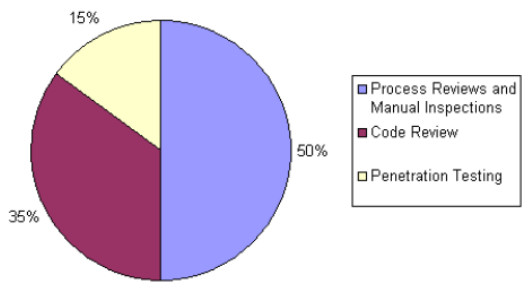
\includegraphics[scale=0.6]{pics/effort.png}
			\end{figure}

	\clearpage
	\section{Security Requirements}

		\subsection{Test Derivation}

		{\bf Testing Objectives} \\
		One of the objectives of security testing is to validate that security controls function as 
		expected. This is documented via {\bf security requirements} that describe the functionality 
		of the security control. At a high level, this means proving confidentiality, integrity, and 
		availability of the data as well as the service. The other objective is to validate that security
		controls are implemented with few or no vulnerabilities. These are common vulnerabilities, 
		such as the OWASP Top Ten, as well as vulnerabilities that are previously identified with 
		security assessments during the SDLC, such as threat modeling, source code analysis, and 
		penetration test. \\

		{\bf Security Requirement Documentation} \\
		The first step in the documentation of security requirements is to understand the 
		business requirements. A {\bf business requirement document} could provide the initial, 
		high-level information of the expected functionality for the application. For example, 
		the main purpose of an application may be to provide financial services to customers or 
		shopping and purchasing goods from an on-line catalogue. A security section of the business 
		requirements should highlight the need to protect the customer data as well as to comply 
		with applicable security documentation such as regulations, standards, and policies.

		Applicable {\bf industry standards} for security need also to be captured by the general security 
		requirement checklist. For example, in the case of applications that handle customer credit 
		card data, the compliance with the PCI DSS standard forbids the storage of PINs and CVV2 data.

		Another section of the checklist needs to enforce general requirements for compliance with the 
		{\bf organization information security standards and policies}. From the functional requirements 
		perspective, requirement for the security control needs to map to a specific section of the 
		information security standards. An example of such requirement can be: {\bf "a password
		complexity of six alphanumeric characters must be enforced by the authentication controls 
		used by the application."} \\

		{\bf Security Requirements Validation} \\
		From the functionality perspective, the validation of security requirements is the main objective of 
		security testing, while, from the risk management perspective, this is the objective of information 
		security assessments. More in depth, the security assessment objective is risk analysis, such
		as the identification of potential weaknesses in security controls that ensure the confidentiality, 
		integrity, and availability of the data. 
		Assuming encryption is used to protect the data, encryption algorithms and key
		lengths need to comply with the {\bf organization encryption standards}. For example, a security 
		requirement that can be security tested is verifying that only allowed ciphers are used 
		(e.g., SHA-1, RSA, 3DES) with allowed minimum key lengths (e.g., more than 128 bit for symmetric 
		and more than 1024 for asymmetric encryption).

		From the security assessment perspective, security requirements can be validated at different 
		phases of the SDLC by {\bf using different artifacts and testing methodologies}. For example, threat 
		modeling focuses on identifying security flaws during design, secure code analysis and reviews 
		focus on identifying security issues in source code during development, and penetration testing 
		focuses on identifying vulnerabilities in the application during testing/validation.

		{\bf Threats and Countermeasures Taxonomies}\\
		A {\bf threat and countermeasure classification} that takes into consideration root causes of 
		vulnerabilities is the critical factor to verify that security controls are designed, coded, 
		and built so that the impact due to the exposure of such vulnerabilities is mitigated.

		The focus of a threat and countermeasure {\bf categorization} is to define security requirements 
		in terms of the threats and the root cause of the vulnerability. The root cause can be 
		categorized as security flaw in design, a security bug in coding, or an issue due to insecure 
		configuration. 	A threat and countermeasure categorization for vulnerabilities can also be used to 
		document security requirements for secure coding such as secure coding standards. An example of 
		a common coding error in authentication controls consists of applying an hash function to encrypt a 
		password, without applying a seed to the value. 


		{\bf Security Testing and Risk Analysis}\\
		By combining the results of source code analysis and penetration testing it is possible to determine 
		the likelihood and exposure of the vulnerability and calculate the risk rating of the vulnerability. 
		For example, high and medium risk vulnerabilities can be prioritized for remediation, while low risk 
		can be fixed in further releases.
		By considering the threat scenarios exploiting common vulnerabilities it is possible to identify 
		potential risks for which the application security control needs to be security tested. By thinking 
		in terms of threats and vulnerabilities, it is possible to devise a battery of tests that simulate 
		such attack scenarios.


		\subsection{Positive Requirements}
			From the perspective of functional security requirements, the applicable standards, policies 
			and regulations drive both the need of a type of security control as well as the control  
			functionality. These requirements are also referred to as {\bf “positive requirements”}, 
			since they state the expected functionality that can be validated through security tests. 
			Examples of positive requirements are: 
				\begin{itemize}
					\item The application will lockout the user after six failed logon attempts.
					\item Passwords need to be six min characters, alphanumeric.
				\end{itemize}
			The validation of positive requirements consists of asserting the expected functionality and, 
			as such, can be tested by re-creating the testing conditions, and by running the test according 
			to predefined inputs and by asserting the expected outcome as a fail/pass condition.
			In order to validate security requirements with security tests, security requirements need to 
			be function driven and highlight the expected functionality {\bf (the what)} and implicitly 
			the implementation {\bf (the how)}. Examples of high-level security design requirements for 
			authentication can be:

				\begin{itemize}
					\item Protect user credentials and shared secrets in transit and in storage
					\item Mask any confidential data in display (e.g., passwords, accounts)
					\item Lock the user account after a certain number of failed login attempts
					\item Do not show specific validation errors to the user as a result of failed logon
					\item Only allow passwords that are alphanumeric, include special characters and six 
				\end{itemize}

		\subsection{Negative Requirements}
			Security tests need also to be risk driven, that is they need to validate the application for 
			unexpected behavior. These are also called {\bf “negative requirements”}, since they specify 
			what the application should not do. Examples of "should not do" (negative) requirements are:
				\begin{itemize}
					\item The application should not allow for the data to be altered or destroyed
					\item The application should not be compromised or misused for unauthorized financial 
					transactions by a malicious user.
				\end{itemize}

			Negative requirements are more difficult to test, because there is no expected behavior to look for. 
			This might require a threat analyst to come up with unforeseeable input conditions, causes, and 
			effects. This is where security testing needs to be driven by risk analysis and threat modeling. 
			The key is to document the threat scenarios and the functionality of the countermeasure as a factor 
			to mitigate a threat. For example, in case of authentication controls, the following security
			requirements can be documented from the threats and countermeasure perspective:

				\begin{itemize}
					\item Encrypt authentication data in storage and transit to mitigate risk of information
					disclosure and authentication protocol attacks.
					\item Encrypt passwords using non reversible encryption such as using a digest (e.g., HASH) 
					and a seed to prevent dictionary attacks.
					\item Lock out accounts after reaching a logon failure threshold and enforce password 
					complexity to mitigate risk of brute force password attacks
					\item Display generic error messages upon validation of credentials to mitigate risk 
					of account harvesting/enumeration.
				\end{itemize}

			Threat modeling artifacts such as {\bf threat trees and attack libraries} can be useful to derive the 
			negative test scenarios. A threat tree will assume {\bf a root attack} and identify different
			{\bf exploits of security controls} and necessary {\bf countermeasures} that could be validated to 
			be effective in mitigating such attacks.

		\subsection{Use and Misuse Cases}
			Pre-requisite in describing the application functionality is to understand what the application 
			is supposed to do and how. This can be done by describing use cases. {\bf Use cases}, in the 
			graphical form as commonly used in software engineering, show the interactions of actors and 
			their relations, and help to identify the actors in the application, their relationships, the
			intended sequence of actions for each scenario, alternative actions, special requirements, 
			and pre- and post-conditions.

			Similar to use cases, {\bf misuse and abuse cases} describe unintended and malicious use scenarios 
			of the application. These misuse cases provide a way to describe scenarios of how an attacker 
			could misuse and abuse the application. By going through the individual steps in a use scenario 
			and thinking about how it can be maliciously exploited, potential flaws or aspects of the application 
			that are not well-defined can be discovered. The key is to describe all possible or, at least, the
			most critical use and misuse scenarios. Misuse scenarios allow the analysis of the application from 
			the {\bf attacker's point of view}.

			\clearpage
			{\bf Sequrity Requirements Derivation Through Use and Misuse Cases:}
				\begin{itemize}
					\item Step 1: Describe the Functional Scenario: 
					\item Step 2: Describe the Negative Scenario: 
					\item Step 3: Describe Functional and Negative Scenarios With Use and Misuse Case:
					\item Step 4: Elicit The Security Requirements. These security requirements need to be 
					documented and tested.

				\end{itemize}

			\begin{figure}[H]
				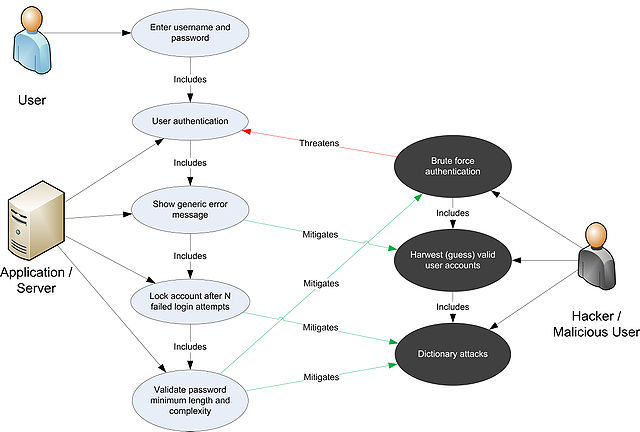
\includegraphics[width=\textwidth]{pics/useAndMisuse.jpg}
			\end{figure}
	\clearpage
	\section{Security Tests Integrated in Developers and Testers Workflow}

		\subsection{ Developers' Security Testing Workflow}
			Security testing during the development phase of the SDLC represents the first 
			opportunity for developers to ensure that individual software components that they 
			have developed are security tested before they are integrated with other components 
			and built into the application. Software components might consist of software artifacts 
			such as functions, methods, and classes, as well as application programming interfaces, 
			libraries, and executables. For security testing, developers can rely on the results of 
			{\bf the source code analysis} to verify statically that the developed source code does 
			not include potential vulnerabilities and is compliant with the secure coding standards. 
			{\bf Security unit tests} can further verify dynamically (i.e., at run time) that the 
			components function as expected.
		\subsection{Testers' Security Testing Workflow}
			After components and code changes are tested by developers and checked in to the application 
			build, the most likely next step in the software development process workflow is to perform 
			tests on the application as a whole entity. This level of testing is usually referred to as 
			{\bf integrated test} and {\bf system level test}. 
			These security tests on the application include both {\bf white box testing}, such as source 
			code analysis, and {\bf black box testing}, such as penetration testing. {\bf Gray box testing} 
			is similar to Black box testing. In a gray box testing we can assume we have some partial 
			knowledge about the session management of our application, and that should help us in 
			understanding whether the logout and timeout functions are properly secured.
			A testing engineer who validates the security of the application in the integrated system 
			environment might release the application for testing in the operational environment 
			(e.g., {\bf user acceptance tests}). The application {\bf functional testing} is usually 
			a responsibility of {\bf QA testers}, while {\bf white-hat hackers/security consultants} 
			are usually responsible for {\bf security testing}. 

	\clearpage
	\section{Security Test Data Analysis And Reporting}

	\subsection{Goals for Security Test Metrices and Measurements}
		The definition of the goals for the security testing metrics and measurements is a pre-requisite 
		for using security testing data for risk analysis and management processes. For example, a 
		measurement such as the {\bf total number of vulnerabilities found} with security tests might quantify 
		the security posture of the application. These measurements also help to identify security 
		objectives for software security testing: for example, reducing the number of vulnerabilities to 
		an acceptable number (minimum) before the application is deployed into production.

		From the perspective of the {\bf effort required to fix} a defect, both security and quality defects 
		can be measured in terms of developer hours to implement the fix, the tools and resources required 
		to fix, and, finally, the cost to implement the fix.

		Security testing data needs to support the security risk strategy at critical checkpoints during 
		the SDLC. For example, vulnerabilities found in source code with source code analysis represent 
		an initial measure of risk. Such {\bf measure of risk (e.g., high, medium, low)} for the vulnerability 
		can be calculated by determining the exposure and likelihood factors and, further, by validating 
		such vulnerability with penetration tests. The risk metrics associated to vulnerabilities found 
		with security tests empower business management to make {\bf risk management decisions}, such as to 
		decide whether risks can be accepted, mitigated, or transferred at different levels within the 
		organization.

		We need to lowering the cost of fixing the vulnerabilities, since it is less expensive to deal with the 
		vulnerabilities when they are found (in the same phase of the SDLC), rather than fixing them 
		later in another phase.

		When security test data is reported it has to provide metrics to support the analysis. The scope 
		of the analysis is the interpretation of test data to find clues about the security of the software 
		being produced as well the effectiveness of the process. Some examples of clues supported by security 
		test data can be:

		Are vulnerabilities reduced to an acceptable level for release? Are all security test requirements being met?
		What are the major root causes of security issues? Which security activity is most effective in finding vulnerabilities? Which team is more productive in fixing security defects and vulnerabilities? 
		Which percentage of overall vulnerabilities are high risks? Which tools are most effective in detecting security vulnerabilities?

		\subsection{Reporting Requirements}

			The security posture of an application can be characterized from the perspective of the effect, 
			such as number of vulnerabilities and the risk rating of the vulnerabilities, as well as from 
			the perspective of the cause (i.e., origin) such as coding errors, architectural flaws, and 
			configuration issues.

			When reporting security test data, the best practice is to include the following information, 
			besides the categorization of each vulnerability by type:
				\begin{itemize}
					\item The security threat that the issue is exposed to
					\item The root cause of security issues (e.g., security bugs, security flaw)
					\item The testing technique used to find it
					\item The remediation of the vulnerability (e.g., the countermeasure)
					\item The risk rating of the vulnerability (High, Medium, Low)
				\end{itemize}

		\subsection{Business Cases}
			For the security test metrics to be useful, they need to {\bf provide value} back to the organization's 
			security test data stakeholders, such as project managers, developers, information security offices,
			auditors, and chief information officers. The value can be in terms of the business case that each 
			project stakeholder has in terms of role and responsibility.

			{\bf Project managers} look for data that allows them to successfully manage and utilize security testing
			activities and resources according to the project plan. 

			To compliance {\bf auditors}, security test metrics provide a level of software security assurance and
			confidence that security standard compliance is addressed through the security review processes 
			within the organization.

			Finally, {\bf Chief Information Officers (CIOs) and Chief Information Security Officers (CISOs)}, 
			responsible for the budget that needs to be allocated in security resources, look for derivation 
			of a {\bf cost/benefit analysis} from security test data to make informed decisions on which security 
			activities and tools to invest. 











